\documentclass{article}

\usepackage{amsmath}
\usepackage{amssymb}
\usepackage{graphicx}
\usepackage[german]{babel}


% For at få faver på texten skal man gå til "Format" og så "Syntax Colering".
% Her kom jeg til https://www.youtube.com/watch?v=Xl1c_1yL47k

\begin{document}

	\title{Assignment 37}
	\author{"pebj, smot"}
	\maketitle

	\begin{enumerate}
		\item Identify all relevant \textbf{Actors}.
		\begin{enumerate}
			\item[Nr.1] Client
			\item[Nr.2] Server
			\item[Nr.3] Moderater
		\end{enumerate}
		\item Identify and describe \textbf{2 non-trivial Scenarios}.
	\end{enumerate}

\begin{tabular}{l r @{} l}
	\multicolumn{2}{c}{} \\
	\hline
	Scenario name	&&Entry sharing\\
	\hline
	Praticipating actor	&&Claus, Jan: Client \\
	instances       	&&\\
	\hline
	Flow of events	&1)&Claus' birthday is coming up, so he needs to invite any participants\\ 
					&&who would like to come. therefore he makes an event in the CALENDAR.\\
				&2)&When Claus have openet CALENDAR, he use the "Add a event" function. which\\ 
					&&to open a new window for spisifikations of the event. \\
				&3)&Then he enters the date, pladse and a shot diskription of the event.\\
					&&Claus also choses a color for the event. a time he like to be alermet\\
					&&of the event and then he confirms his input.\\
				&4)&The CALENDAR closes the spisifikation window and shows Claus calender with\\
					&&hes new event. Claus then use the "Share" function and gets a digital code\\
					&&he copyes and pasts it on hes Facebook wall.\\
				&5)&The friend Jan notices this digital code and wishes to take part in Claus' \\ 
					&&birthday. He therefore uses the digital code to get to a window, where he can\\
					&&chose to accept, which ther vill put the event in his calendar in CALENDAR.\\
				&6)&Jan and Claus can new see the event in ther calendar, with date, place,\\
					&&deskription and how many praticipan ther have acceptet the event.\\
	\hline
\end{tabular}
\\


\begin{tabular}{l r @{} l}
	\multicolumn{2}{c}{} \\
	\hline
	Scenario name	&&Upcomming event notification\\
	\hline
	Praticipating actor	&&Claus: Client \\
	instances       	&&server: Server\\
	\hline
	Flow of events	&1)&A week ago Claus inserted an event to his CALENDAR where he added\\ 
					&&a "event alert" to notifi him 2 hours before the event.\\
				&2)&The server react to the "event alert" at the spisefid time, by sending\\
					&&a message to the Client Claus with the ditails for the upcomming event.\\
				&3)&Claus now gets an message notification from his smartphone\\ 
					&&which he then uses to read the message.\\
				&4)&The messagel tells him of the upcomming event and show him hes calender\\
					&&for today.\\
	\hline
\end{tabular}

	\begin{enumerate}
		\item[3.] Identify all  relevant \textbf{Use Cases} and draw the \verb= "sticky man" UML= diagram.\\
		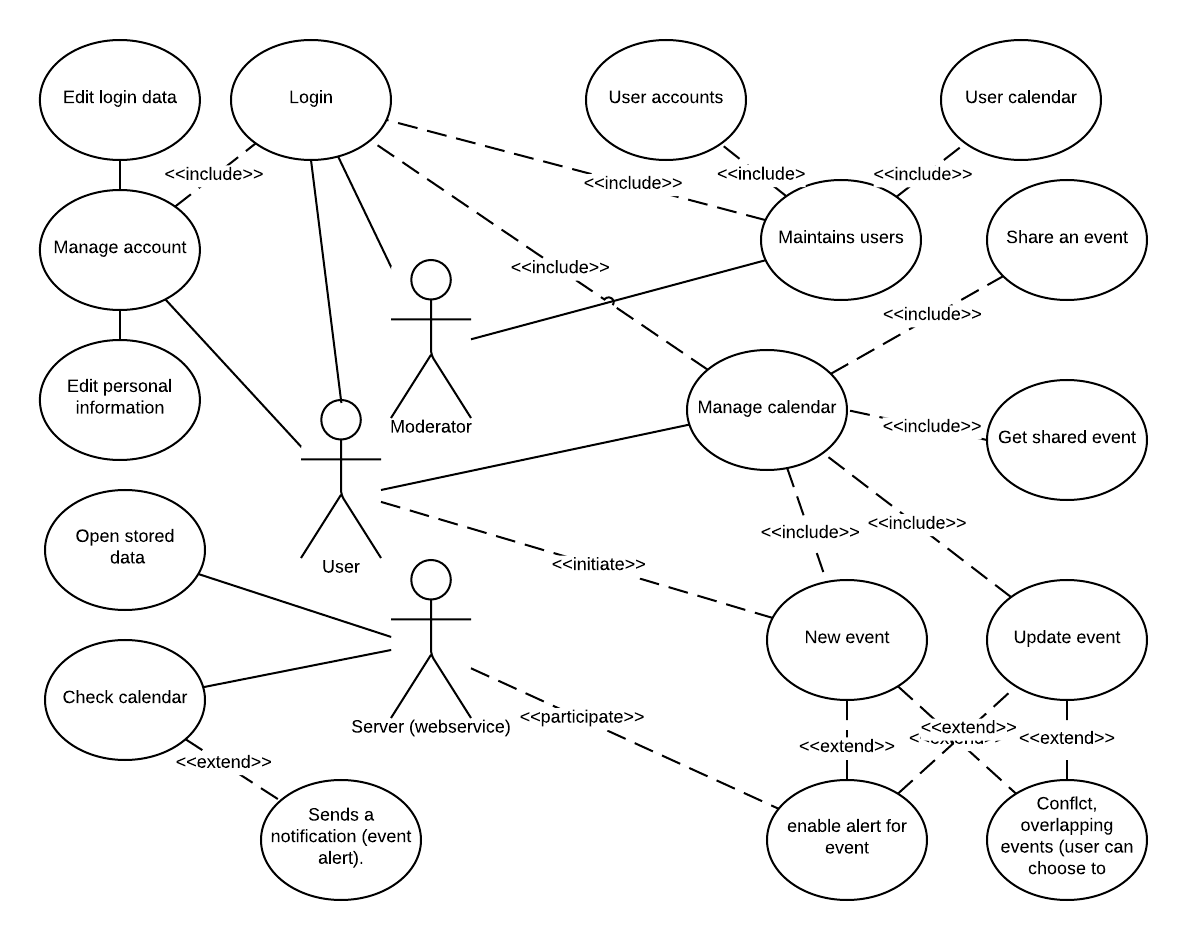
\includegraphics[scale = 0.38]{C:/Users/stin7054/Documents/GitHub/BDSA2014/LatexAS.37/UserCases.png}\\
		\pagebreak{}
		\item[4.] Select 3 \textbf{non-trivial Use Cases} and document them using the use case table\\
	\end{enumerate}
\begin{tabular}{l r @{} l}
	\multicolumn{2}{c}{} \\
	4.1&&\\
	\hline
	Use case name:	&&Edit personal information\\
	\hline
	Participating actors:&&User \\
	\hline
	Flow of events:	&1.&User chooses to manage his account.\\
				&2.&User chooses to edit his/hers personal information.\\
	\hline
	Entry condition:	&&User is logged into the system.\\
	\hline
	Exit condition:	&&The user updates his personal information.\\
	\hline
\end{tabular}
	\\
	.\\
\begin{tabular}{l r @{} l}
	\multicolumn{2}{c}{} \\
	4.2&&\\
	\hline
	Use case name:	&&Enable alert\\
	\hline
	Participating actors:&&User, Server \\
	\hline
	Flow of events:	&1.&User chooses to manage his calendar (login include has been profiled\\
				&2.&by entry condition). User chooses to add a new event.\\
				&3.&User chooses to enable an alert for his event (explained by the \flqq extend\frqq\\
					&& which tells us its an extension of the base case. You have to do the base case,\\
					&& but you may do the extension).\\
				&4.&The user chooses to enable the notification alert (due to the server participating\\
					&& in this, the server will act as an observer to your choice of enabling the event).\\
				&5.&You enable the alert and the server will know the result.\\
	\hline
	Entry condition:	&&User is logged into the system.\\
	\hline
	Exit condition:	&&The user chooses to enable/disable the alert.\\
	\hline
\end{tabular}
	\\
	.\\
\begin{tabular}{l r @{} l}
	\multicolumn{2}{c}{} \\
	4.3&&\\
	\hline
	Use case name:	&&Send event alert\\
	\hline
	Participating actors:&&Server\\
	\hline
	Flow of events:	&1.&Server checks the events for all users.\\
				&2.&On the condition that it finds an upcoming event, we will end up sending\\
					&&a notification to the user about it (using \flqq extend\frqq, we say\\
					&&that we arrive there as a condition is met,\\
					&&in this case, an event is an upcoming event).\\
	\hline
	Entry condition:	&&A timed loop chooses to have the server perform this task regularly.\\
	\hline
	Exit condition:	&&Event alerts have been sent for all upcoming events.\\
	\hline
\end{tabular}

	\pagebreak{}

\begin{enumerate}
		\item[5.] Identify \textbf{Relationships} between Actors and Use Cases and finalize the \verb= "sticky man"=  diagram\\
		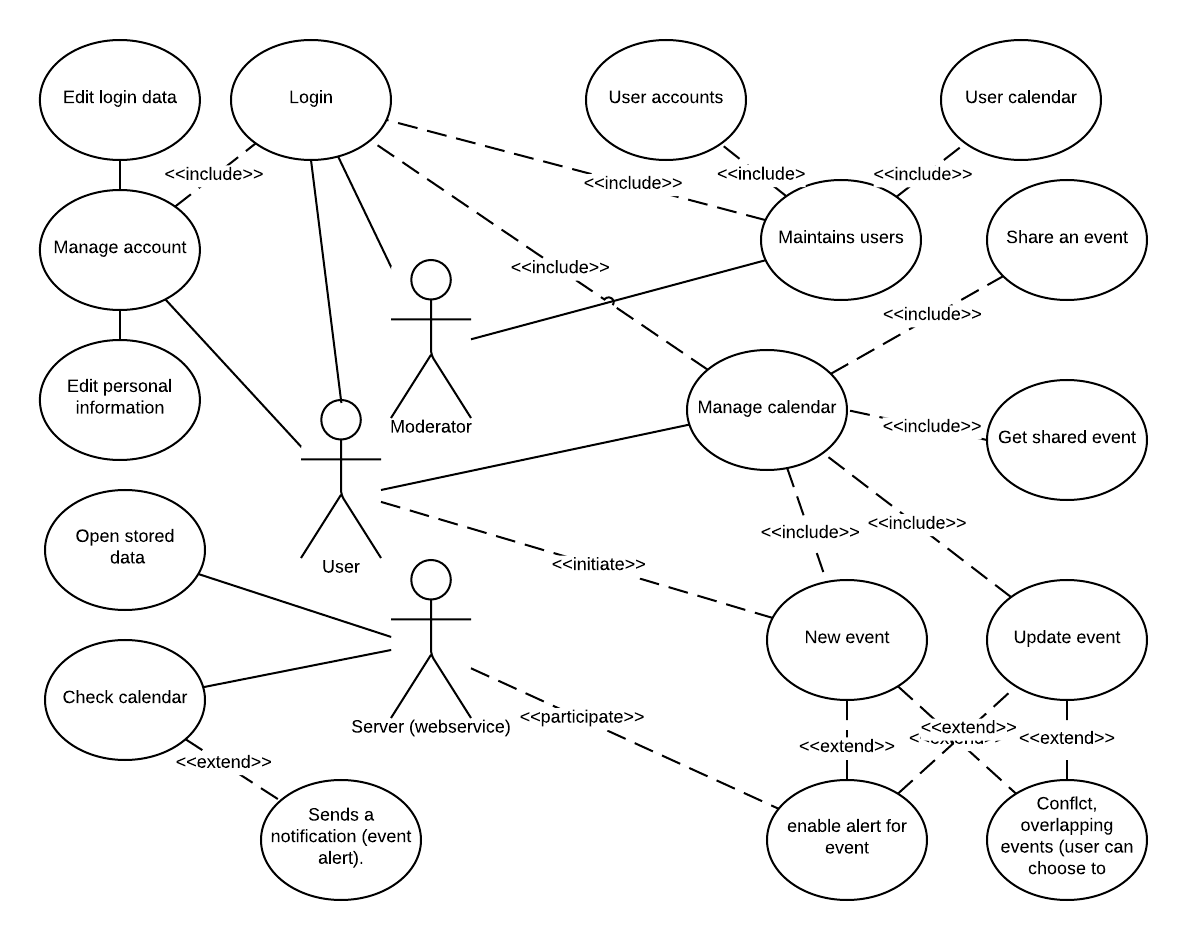
\includegraphics[scale = 0.38]{C:/Users/stin7054/Documents/GitHub/BDSA2014/LatexAS.37/UserCases.png}\\
		\pagebreak{}
		\item[6.] Identify \textbf{Initial Analysis Objects} and document them in a table\\
\end{enumerate}

\begin{tabular}{l r @{} l}
	\textbf{Participating objects for the enable alert use case.}\\
	\hline
	\textbf{Server (web service):} Web service running on a server which regularly checks up on all events and \\
	notifies users in case of an upcoming event. It is up to the user if he wants to have a notification sent,\\ 
	so the server will participate in the user’ events and choice of enabling the notification alert.\\
	\hline
	\textbf{User} the user can create events in his calendar. As such he is the initiator of event creation and \\
	other users may participate in those events. \\
	Additionally a new possible event alert may be initiated which a server will participate in.\\
	\hline
\end{tabular}
	\\

\begin{enumerate}
		\item[7.] Identify \textbf{Non-functional Requirements} and document them i a table\\
\end{enumerate}

\begin{tabular}{l r @{} l}
	\textbf{Non-functional Requirements}\\
	\hline
	\textbf{Usability:} Users must be able to view (not edit) a shared event without having an account\\
	 and without logging in. The user interface should be kept simple thus fancy features should be kept\\
	 at a minimum. The only exception to the latter is if more features are kept isolated\\ 
	 from the simple interface, meaning that there may be a page dedicated for advanced features.\\
	\hline
	\textbf{Reliability:} The system may not make changes to the database in a way where a failure\\
	 could corrupt the database. For instance, a script may not make multiple statements that depend\\
	 on each other and send them to the server individually, only collectively.\\
	\hline
	\textbf{Performance:} The asymptotic running time of the program must not increase propositionally\\
	by the number of events.\\
	\hline
	\textbf{Supportability:} The system must be designed in a way, so that new notifications types besides\\
	upcoming events notification can be implemented without the need to alter the implementation\\
	of the upcoming event notification.\\
	\hline
	\textbf{Implementation:} The implementation must work on\\
	at least one of the following main platform: Windows or Mac OS.\\
	\hline
	\textbf{Operation:} moderator maintains the users, but should be kept from seeing as much personal\\
	 information from users as possible unless specifically requested by the moderator.\\
	\hline
	\textbf{Legal:}  As in accordance to the Danish law § 264,\\
	 it is not legal to forward messages or pictures concerning another person’ private circumstances\\
	 or pictures without permission from the person in question.\\ 
	This also means that the calendar system must not publicize/distribute the user’ events\\
	 or personal information (to the front page of the website etc.) without the user’ personal permission.\\
	\hline
\end{tabular}

\end{document}